\documentclass{report}


%%%%%%%%%%%%%%%%%%
%   Liste des packages utilisés  %
%%%%%%%%%%%%%%%%%%

\usepackage{amssymb}
\usepackage{array}
\usepackage{booktabs}
\usepackage{multirow}
\usepackage{float}
\usepackage{lmodern} %Pack de police
\usepackage{color}
\usepackage[dvipsnames]{xcolor}
\usepackage{graphicx}
\usepackage{svg}
\usepackage[utf8x]{inputenc}
\usepackage[T1]{fontenc}
%\usepackage{natbib}
\usepackage[square,sort,comma,numbers]{natbib}
\usepackage[francais,english]{babel}
\usepackage{caption}
\usepackage{listings}
\usepackage{booktabs}
\usepackage[top=2cm, bottom=2cm,left=2cm, right=2cm]{geometry}
\usepackage{blindtext}
\usepackage{setspace}
\usepackage{graphicx}
\usepackage{sidecap}
\usepackage{titlesec, blindtext, color} % titres spéciaux + couleur pour les chapter
\usepackage{fancyhdr}
\usepackage{seqsplit}
\usepackage[hyphens]{url}
\usepackage{lipsum}  
\usepackage{soul}

% on transforme les chapters en juste le numéro suivi du titre, avec un barre grisse
\definecolor{gray75}{gray}{0.75}
\newcommand{\hsp}{\hspace{20pt}}
\titleformat{\chapter}[hang]{\Huge\bfseries}{\thechapter\hsp\textcolor{gray75}{|}\hsp}{0pt}{\Huge\bfseries}


%\titleformat{\chapter}[display]
%	{\normalfont\huge\bfseries}{}{0pt}{\Huge}

\titlespacing*{\chapter}{0pt}{0pt}{15pt}
\titlespacing*{\subsection}{0pt}{2.0ex plus 1ex minus .2ex}{0.5ex plus .2ex}
\titlespacing*{\subsubsection}{0pt}{1.0ex plus 1ex minus .2ex}{0.5ex plus .2ex}


\makeatletter
\newcommand\footnoteref[1]{\protected@xdef\@thefnmark{\ref{#1}}\@footnotemark}
\makeatother


%Définition du style des bords de page
\pagestyle{fancy}
\renewcommand{\chaptermark}[1]{\markboth{\bsc{\thechapter{}- } #1}{}}
\lhead{}
\chead{}
\rhead{\leftmark}
\cfoot{}
\rfoot{Page \thepage}

\fancypagestyle{plain}{%
    \lhead{}
    \chead{}
    \rhead{}
    \renewcommand{\headrulewidth}{0pt}
    %\lfoot{Groupe n\up{o}2}
    \cfoot{}
    \rfoot{Page \thepage}
}

\begin{document}

\begin{titlepage}


\textbf{Le Mans Université}
\begin{flushright}
\hspace{6cm} \textit{UFR Sciences et Techniques}
\\
\textit{Département Informatique}
\end{flushright}

\vskip1cm
\begin{center}
%% Pour redéfinir la distance entre la boite et le texte
\fboxsep6mm
%% Pour redéfinir l'épaisseur de la boite
\fboxrule1.3pt

\vspace{2cm}

%% Le \vphantom{\int_\int} sert à introduire de l'espace entre les deux lignes
%% (essayez donc de le commenter)
$$\fbox{$
  \begin{array}{c}
  \textbf{ANDROID APPLICATION}
  \\
  \textbf{REPORT}
  \vphantom{\int_\int}
  \\
  \textbf{Programmation d'interfaces embarquées}
  \\
  \textbf{Master 1 Informatique}
  \\
  \textbf{2018/2019}
  \\
  \\
  \\
  \textit{Teyssier Titouan, Pelloin Valentin}
  \end{array}
  $}
$$
\end{center}

\vspace{2cm}

\begin{center}
   \vspace{12pt}
   \today
\end{center}

\vspace{4cm}

\begin{figure}[H]
	\centering
    
\includegraphics[width=5cm]{logo.png}
\end{figure}


\end{titlepage}



\tableofcontents


\chapter{Our application : Visual Life Configurator}
Our application is a cellular automaton simulation game. The player is free to create new automatons with the rules we want (for example Conway's game of life, Wireworld, ...).
For each automaton, the player configures how the automaton work, the types of cells, how neighbours are calculated, and the rules for a cell to be transformed into another one.\\
Then, the player can create as many worlds he wants, edit them, and play with them.\\
Our application is called \texttt{VLC}, it stands for Visual Life Configurator.

\section{Persona}

\paragraph{Name}
John Doe
\paragraph{Age}
21
\paragraph{About}
John studies computer science. He is interested into algorithms and life simulation. John likes playing games on his phone while waiting for his bus while going to the University.
\paragraph{Goals}
\begin{itemize}
\item Learn new things
\item Build things with Legos
\end{itemize}

\section{User stories}
\begin{itemize}
	\item As a player, I want to entertain myself by playing a game ;
	\item As a player, I want to learn new automaton rules ;
	\item As a player, I want to experiment new configurations of cellular automatons ;
	\item As a player, I want to express myself by creating and building worlds
\end{itemize}

\chapter{Functional study}

\section{Storyboards}

Below, the mock-ups of our application:
\vspace{12pt}

\begin{minipage}{.45\textwidth}
  \begin{minipage}{.45\linewidth}
    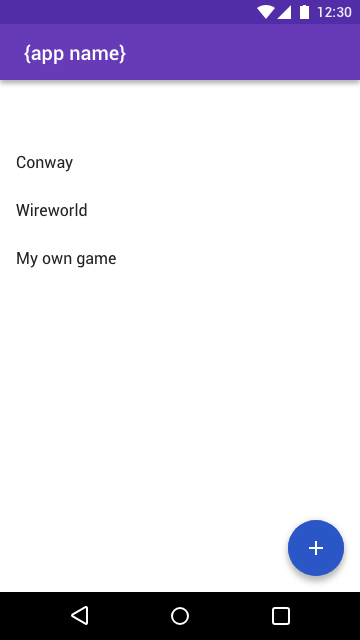
\includegraphics[width=\linewidth]{../mock-ups/Home.png}
  \end{minipage}\hfill
  \begin{minipage}{.45\linewidth}
    \captionof{figure}{The main activity of VLC. \\ The player can find all the automatons he created, and click on them to edit them or to play on a game.\\ The player can also click on the "plus" button to create and configure a new automaton.}
  \end{minipage}%
\end{minipage} \hfill
\begin{minipage}{.45\textwidth}
  \begin{minipage}{.45\linewidth}
    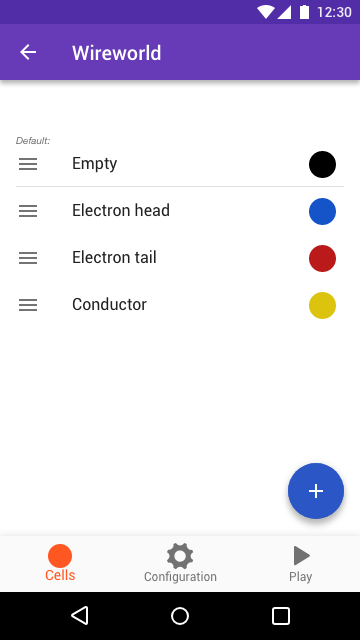
\includegraphics[width=\linewidth]{../mock-ups/Cells.png}
  \end{minipage}\hfill
  \begin{minipage}{.45\linewidth}
    \captionof{figure}{Inside an automaton, cells tab. \\ The player can create and remove cell types for this automaton. He can reorganize the order of the cells. The first cell type is the default one, the type of the cell that will fill the grid when creating a blank world.}
  \end{minipage}%
\end{minipage} \hfill


\begin{minipage}{.45\textwidth}
  \begin{minipage}{.45\linewidth}
    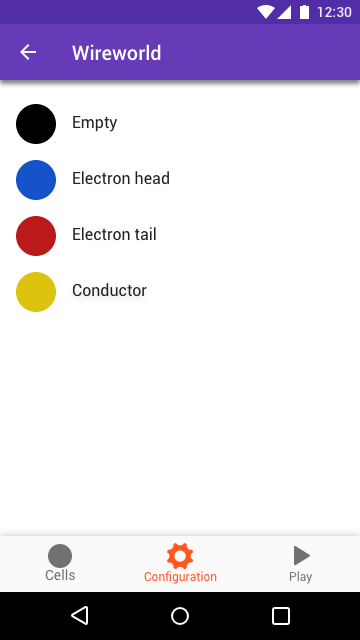
\includegraphics[width=\linewidth]{../mock-ups/Configuration.png}
  \end{minipage}\hfill
  \begin{minipage}{.45\linewidth}
    \captionof{figure}{Inside an automaton, configuration tab. \\ In this tab, the player can access the configuration for each cell.}
  \end{minipage}%
\end{minipage} \hfill
\begin{minipage}{.45\textwidth}
  \begin{minipage}{.45\linewidth}
    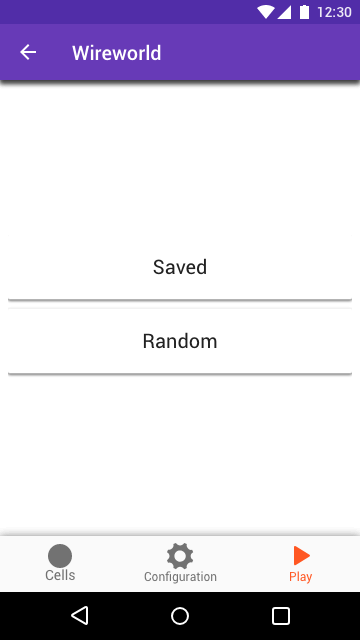
\includegraphics[width=\linewidth]{../mock-ups/Play.png}
  \end{minipage}\hfill
  \begin{minipage}{.45\linewidth}
    \captionof{figure}{Inside an automaton, play tab. \\ In this tab, the user can access to its saved games. He can also choose to play on a random world.}
  \end{minipage}%
\end{minipage} \hfill


\begin{minipage}{.45\textwidth}
  \begin{minipage}{.45\linewidth}
    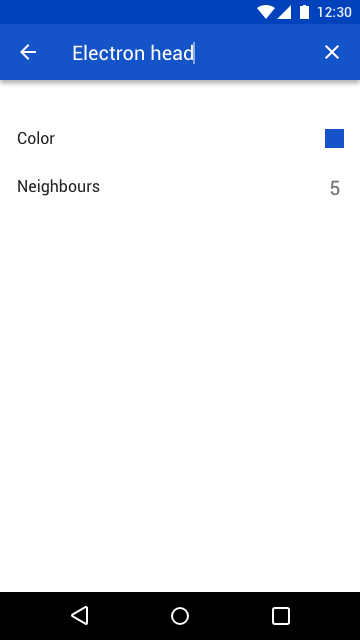
\includegraphics[width=\linewidth]{../mock-ups/Electron_head.png}
  \end{minipage}\hfill
  \begin{minipage}{.45\linewidth}
    \captionof{figure}{Cell parameter activity. \\ For this specific cell type, the user can edit its name, and its color. He can also access to the neighbours choosing screen.}
  \end{minipage}%
\end{minipage} \hfill
\begin{minipage}{.45\textwidth}
  \begin{minipage}{.45\linewidth}
    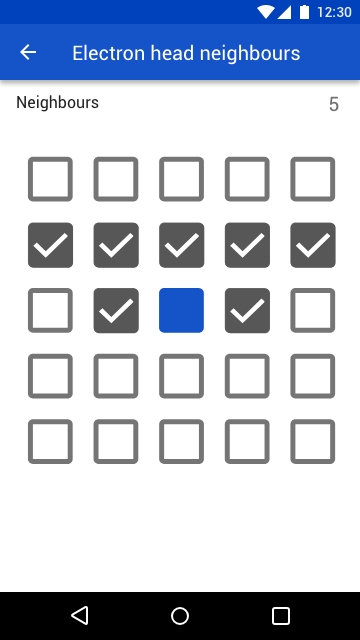
\includegraphics[width=\linewidth]{../mock-ups/Electron_head_neighbours.png}
  \end{minipage}\hfill
  \begin{minipage}{.45\linewidth}
    \captionof{figure}{Cell neighbours choosing. \\ On this activity, the player can choose which cells are being counted by the automaton as neighbours for this specific cell type.}
  \end{minipage}%
\end{minipage} \hfill


\begin{minipage}{.45\textwidth}
  \begin{minipage}{.45\linewidth}
    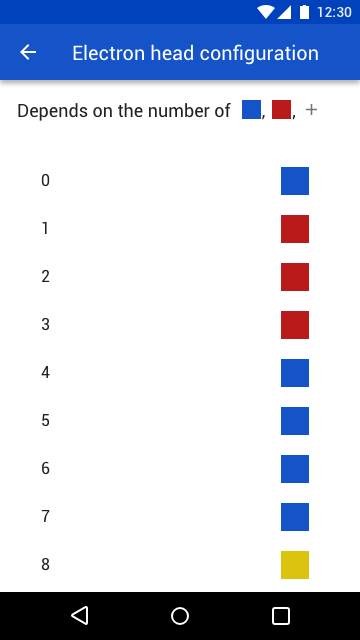
\includegraphics[width=\linewidth]{../mock-ups/Electron_head_configuration.png}
  \end{minipage}\hfill
  \begin{minipage}{.45\linewidth}
    \captionof{figure}{Cell type rules edition. \\ For this cell type (blue one), the player configured the rules of transformation. For example, if there are 8 neighbours around a blue cell, it will be transformed to a yellow cell in the next generation.}
  \end{minipage}%
\end{minipage} \hfill
\begin{minipage}{.45\textwidth}
  \begin{minipage}{.45\linewidth}
    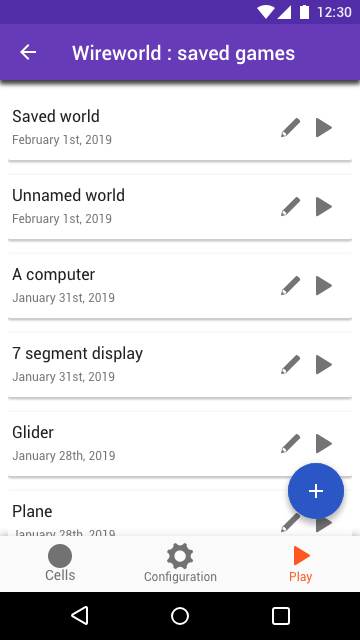
\includegraphics[width=\linewidth]{../mock-ups/Saved.png}
  \end{minipage}\hfill
  \begin{minipage}{.45\linewidth}
    \captionof{figure}{List of saved games. \\ The player can list worlds that are existing for an automaton. For each world, he can edit it, or play on it. By clicking on the "plus" button, he can also create a new blank world.}
  \end{minipage}%
\end{minipage} \hfill


\begin{minipage}{.45\textwidth}
  \begin{minipage}{.45\linewidth}
    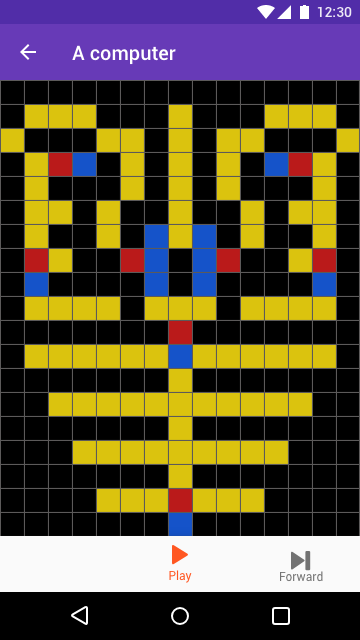
\includegraphics[width=\linewidth]{../mock-ups/Play_game_paused.png}
  \end{minipage}\hfill
  \begin{minipage}{.45\linewidth}
    \captionof{figure}{Playing game activity : paused. \\ By clicking on "Forward", the player can generate the next step.}
  \end{minipage}%
\end{minipage} \hfill
\begin{minipage}{.45\textwidth}
  \begin{minipage}{.45\linewidth}
    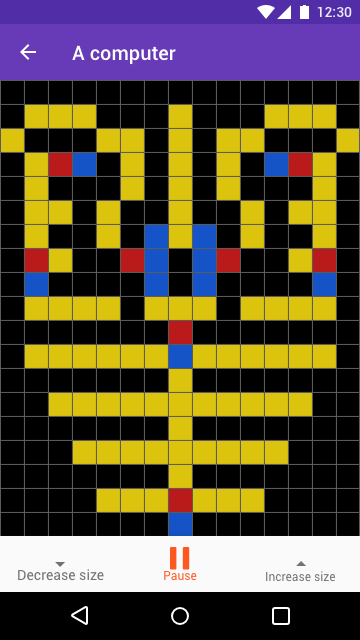
\includegraphics[width=\linewidth]{../mock-ups/Play_game_playing.png}
  \end{minipage}\hfill
  \begin{minipage}{.45\linewidth}
    \captionof{figure}{Playing game activity : playing. \\ The player can zoom in or zoom out.}
  \end{minipage}%
\end{minipage} \hfill


\begin{minipage}{.45\textwidth}
  \begin{minipage}{.45\linewidth}
    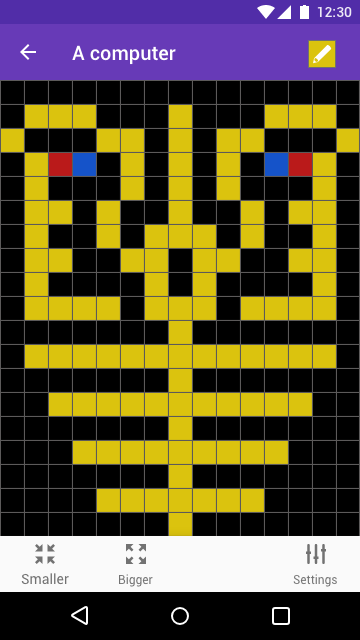
\includegraphics[width=\linewidth]{../mock-ups/Edit_game.png}
  \end{minipage}\hfill
  \begin{minipage}{.45\linewidth}
    \captionof{figure}{Editing a game. \\ The player can drag on cells to color them.}
  \end{minipage}%
\end{minipage} \hfill
\begin{minipage}{.45\textwidth}
  \begin{minipage}{.45\linewidth}
    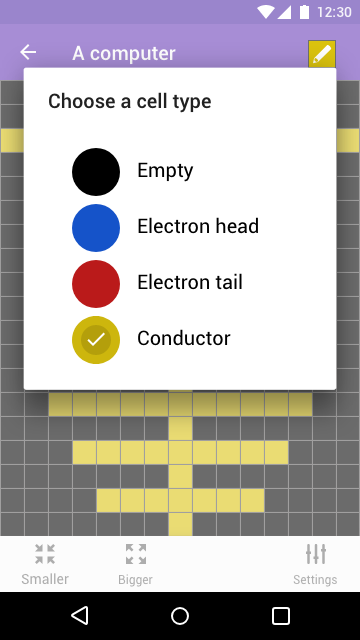
\includegraphics[width=\linewidth]{../mock-ups/Edit_game_popup.png}
  \end{minipage}\hfill
  \begin{minipage}{.45\linewidth}
    \captionof{figure}{Editing a game. \\ The player clicked on the pen in toolbar. He can change the color of cells he will be placing.}
  \end{minipage}%
\end{minipage} \hfill

\vspace{12pt}
A demonstration of these mock-ups can be seen at \url{https://github.com/valentinp72/VisualLifeConfigurator/blob/master/docs/mock-ups/demo.mp4?raw=true}.


\newpage
\section{Architecture}

Our project architecture is based on an MVC (Model-View-Controller) pattern. Below, a class diagram of it.

\begin{figure}[H]
	\centering
	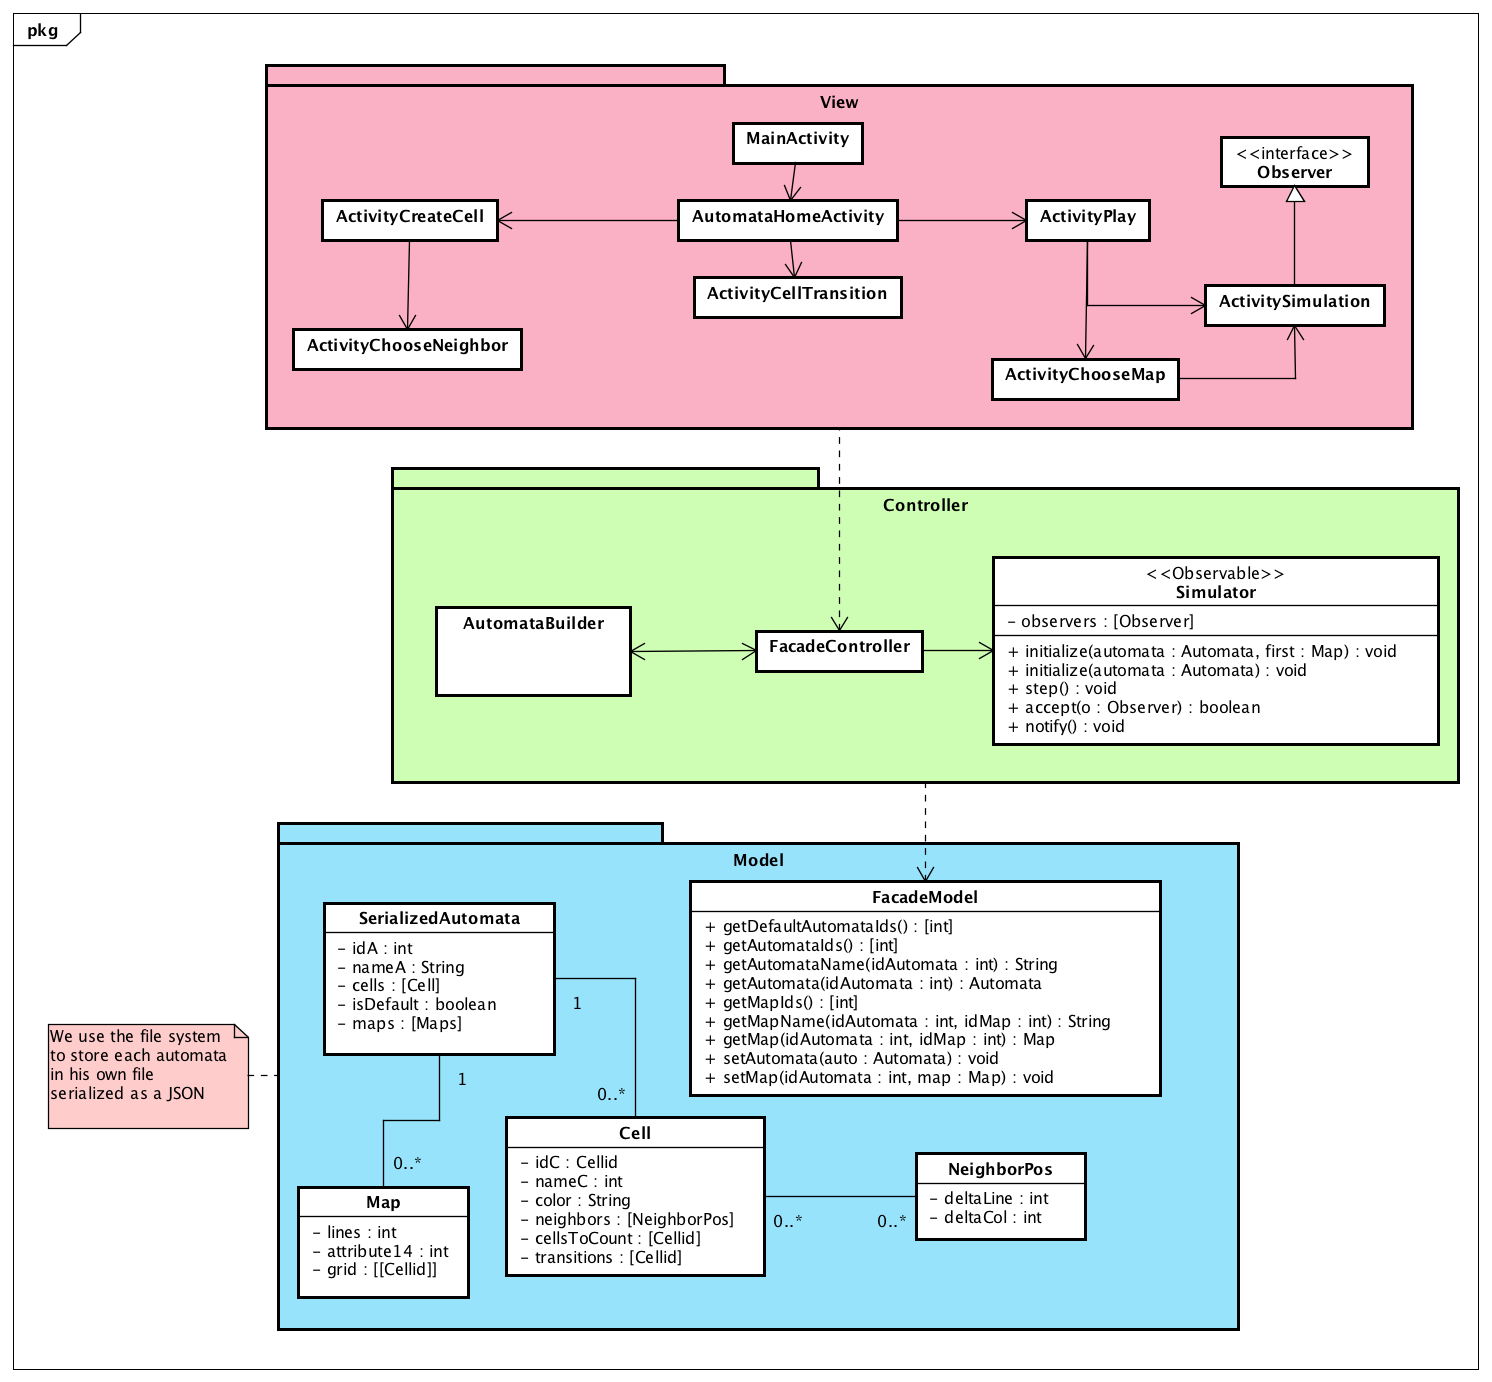
\includegraphics[width=\linewidth]{../class_diagram.png}
	\caption{Class diagram of our application}
\end{figure}

\section{Github link}
Our project is accessible at \url{https://github.com/valentinp72/VisualLifeConfigurator}.


\chapter{Technical details}

\section{Persistence}
\par Our application saves maps and automatons on the phone using internal files. The \texttt{Persistence} class is responsible of loading and saving objects from the device. Automatons are saved in a XML format, whereas Maps contents are saved in plain text files, lowering the size of the files. \\
Default maps and automatons are given in a Asset folder (read-only). When the user needs to reset these games, he can click on a reset button on the home screen.

\section{Data communication between activities}
\par Once loaded, a Map, a Cell or an Automaton is given to the activities needing them as \texttt{Serialized} Extras. With hindsight, everything except Maps should be saved in a SQLite Database. This way, we would not have any problem of modified Serializable objects not being known by every activity. This would also prevent many bugs and many hacks to prevent them from happening, since we actually need to resend some data after edition to other activities, and for some function it does not work (for example when creating a new Automaton or a new Cell).

\section{Simulator operation}
\par The \texttt{Simulator} works by loaded a configured Automaton and Map, and play the map for this Automaton. Since every map can be played with every possible automaton, it is first converted into a compatible map for the given automaton. A \texttt{SimulatorThread} is created for running the game on a loop with interfering with the UI responsiveness. 

\chapter{Achieved work}
\section{Current application status}
\par Currently, the application support loading and saving maps from both the assets and the internal files. Cells can be edited (name, color, neighbours to use) and configured (transitions when a specific number of cells is neighbouring cell type). When editing or configuring a Cell, the toolbar color and status bar color are updated according to the cell color, to allow a better understanding of the application by the user.\\
\par Saved maps are present in the game, and can be played by the user (even maps not initially compatible with the automaton). The user is also allowed to play random maps, even though he is not able to save it for the moment.\\
For the moment, it's also not possible to edit a map before paying it, but it should be rather simple.\\
The application is available French and in English. 

\section{Tasks assignment}
Both Titouan and Valentin did storyboards and architecture study. Programming-wise, Valentin did the user interface and persistence module, whereas Titouan did the back-end operations (maps, automatons, neighbours, simulator, ...).

\chapter{Conclusion}
This project allowed us to learn to create an Android Application that could potentially be published to the public through the Play Store. It showed us how complete and developed Android is, but in the meantime, it disappointed us about some important features (data assets folder that is read-only and internal storage that can't be easily filled with default files for example).  

\chapter{Appendix : application screenshots}
\begin{minipage}{.45\textwidth}
  \begin{minipage}{.45\linewidth}
    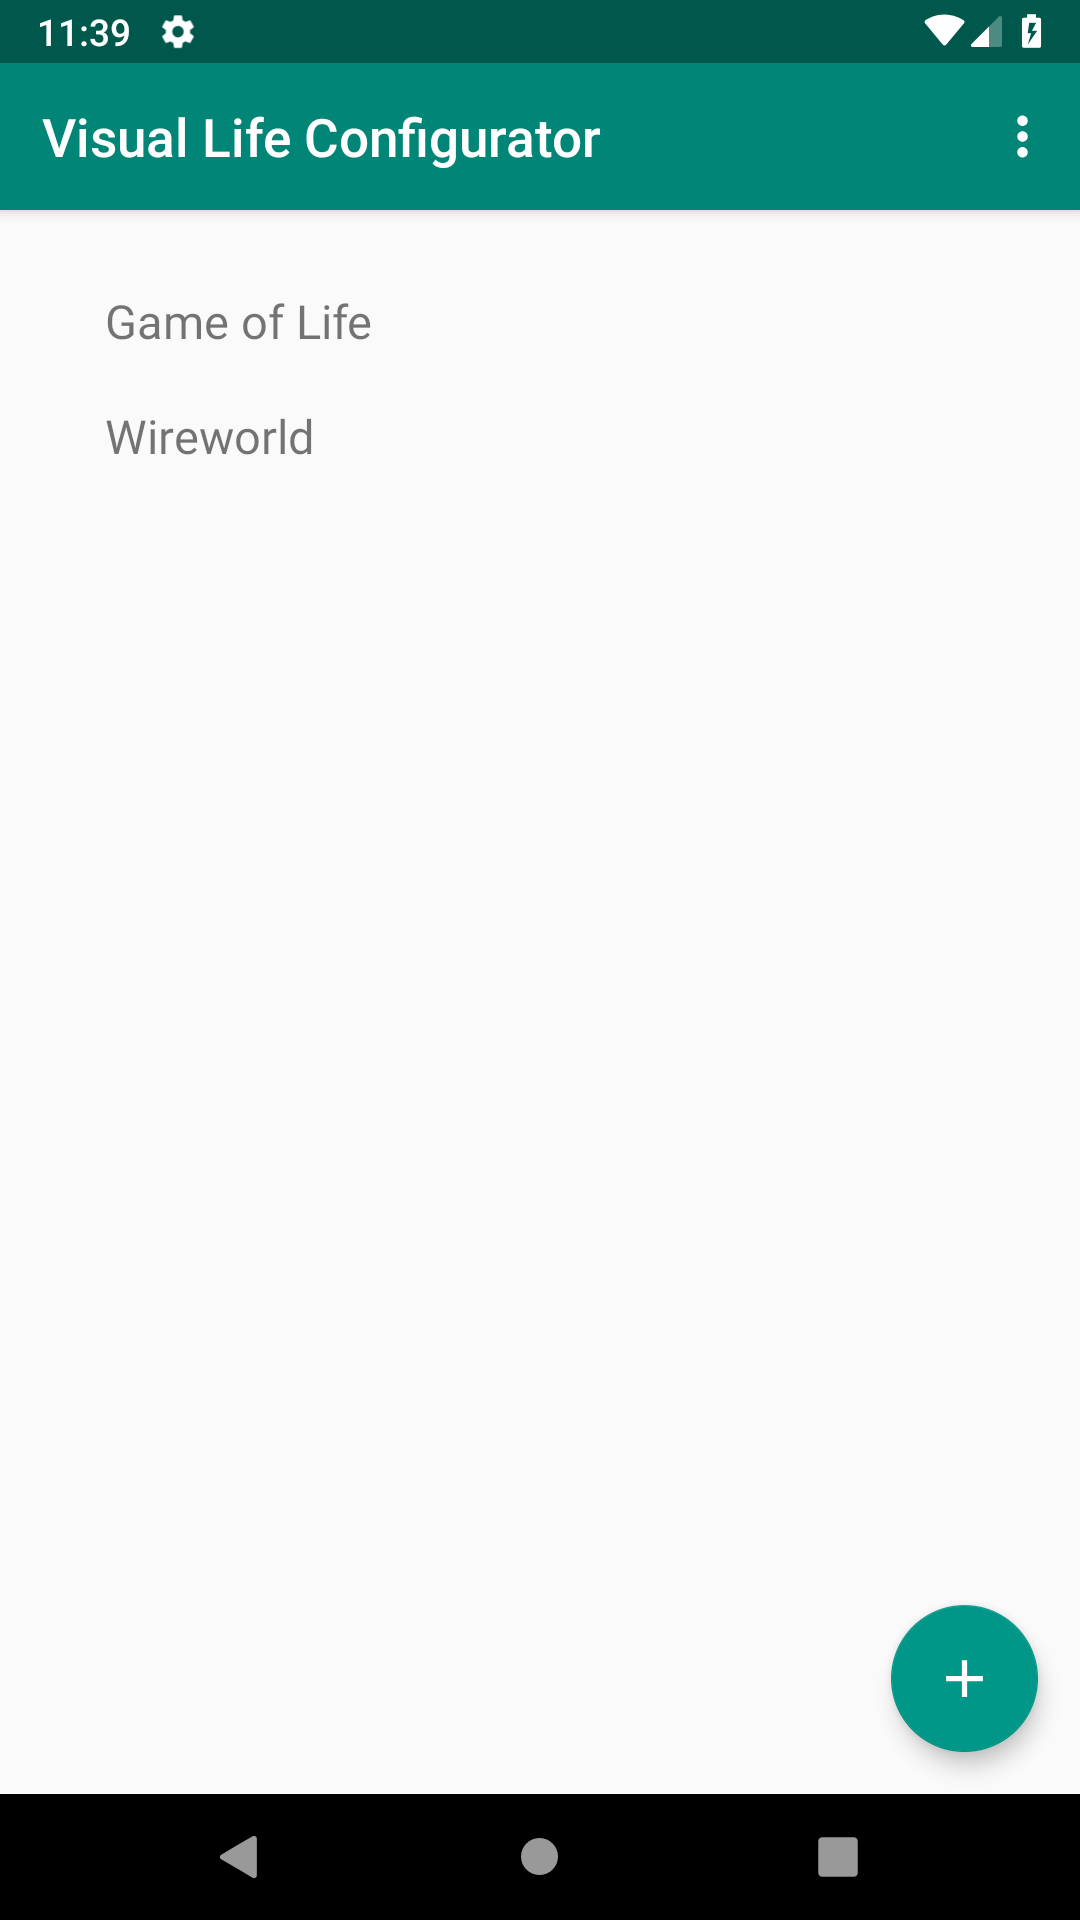
\includegraphics[width=\linewidth]{screens/home.png}
  \end{minipage}\hfill
  \begin{minipage}{.45\linewidth}
    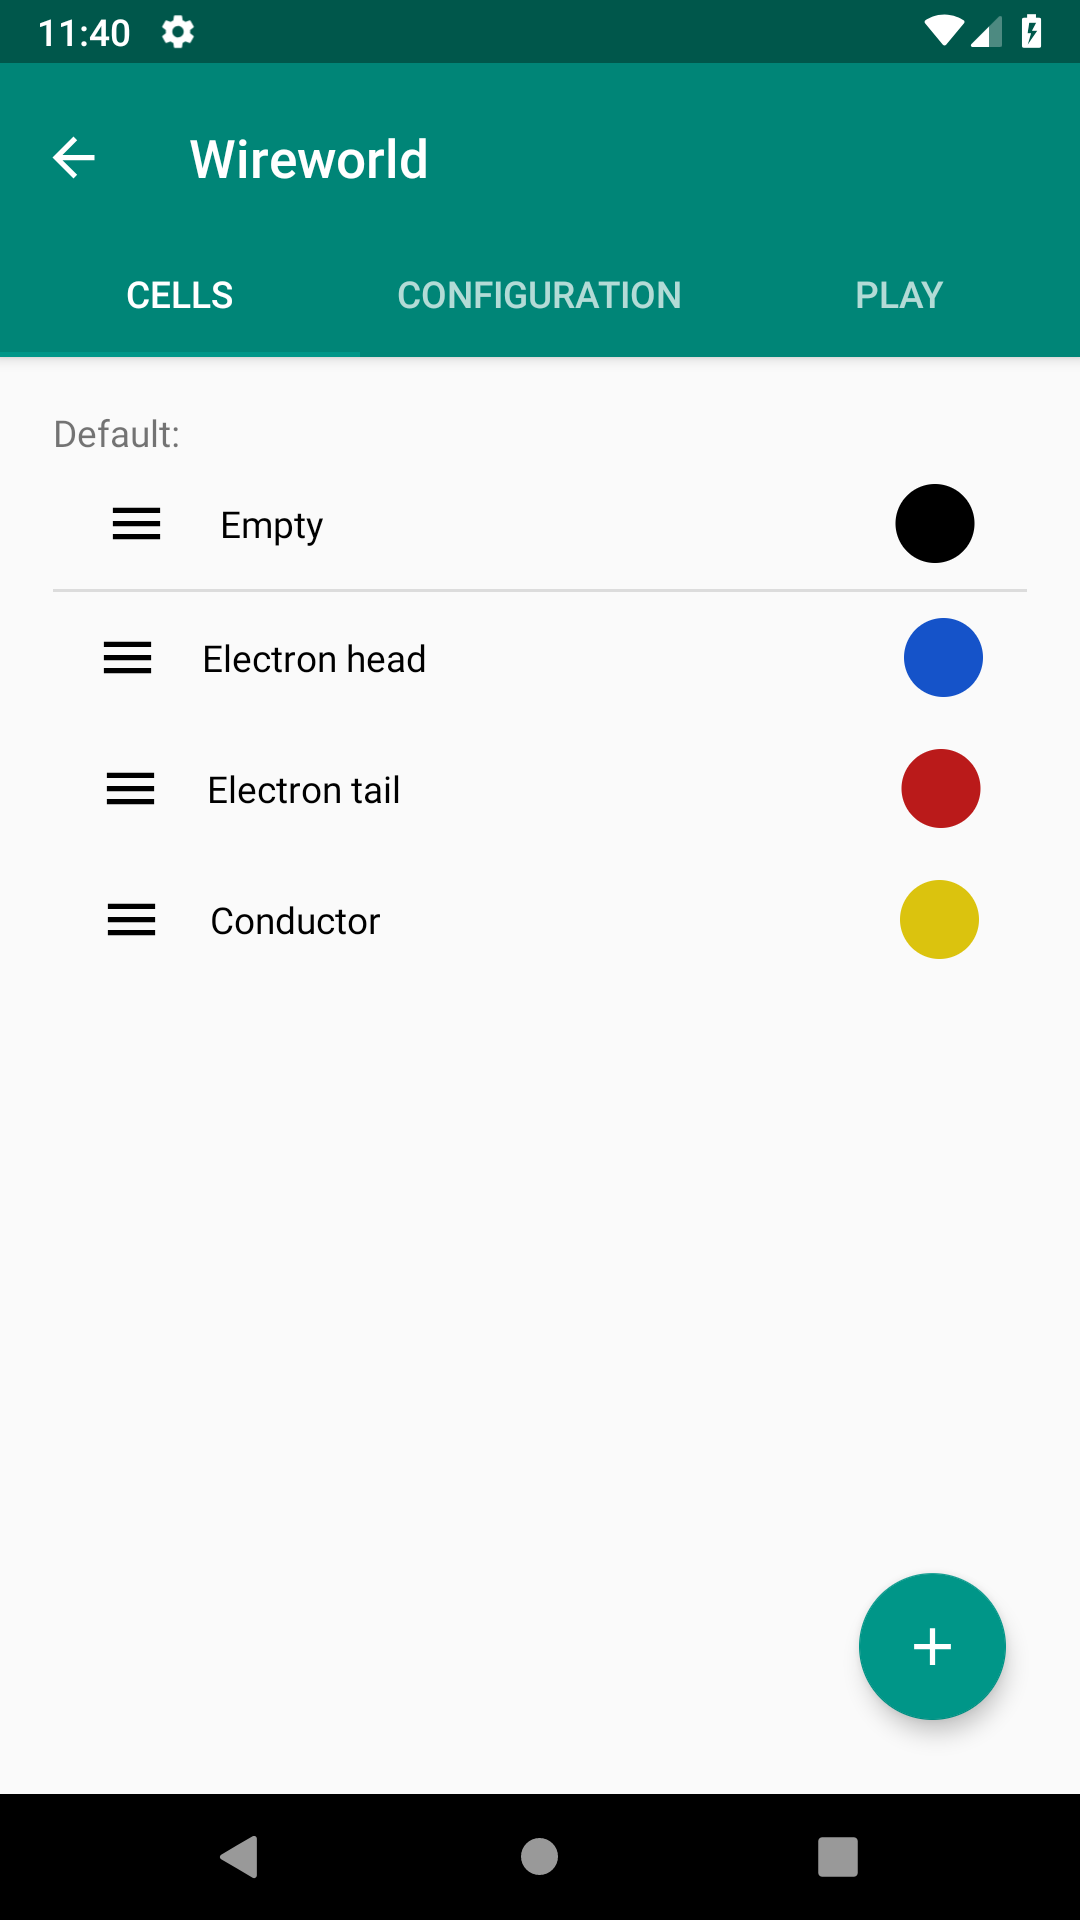
\includegraphics[width=\linewidth]{screens/cells.png}
  \end{minipage}\hfill
\end{minipage} \hfill
\begin{minipage}{.45\textwidth}
  \begin{minipage}{.45\linewidth}
    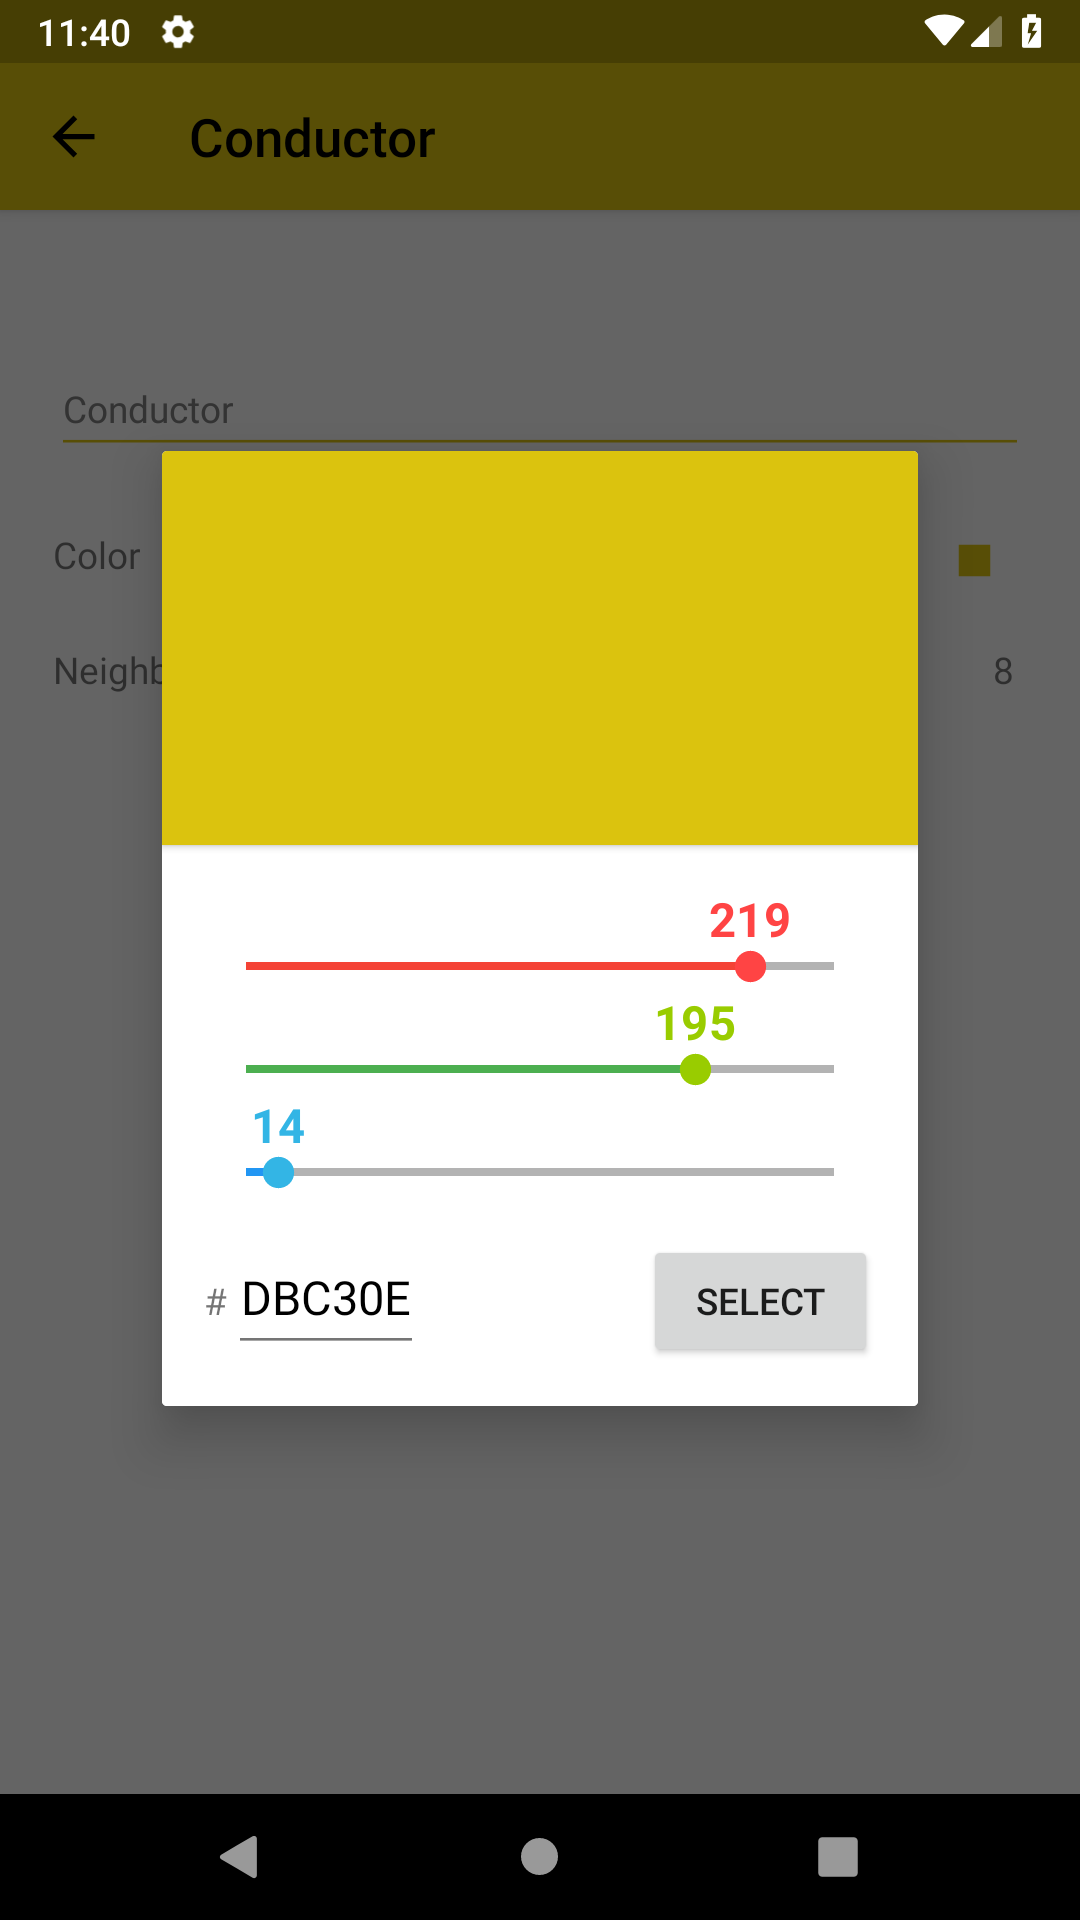
\includegraphics[width=\linewidth]{screens/cell_edit.png}
  \end{minipage}\hfill
  \begin{minipage}{.45\linewidth}
    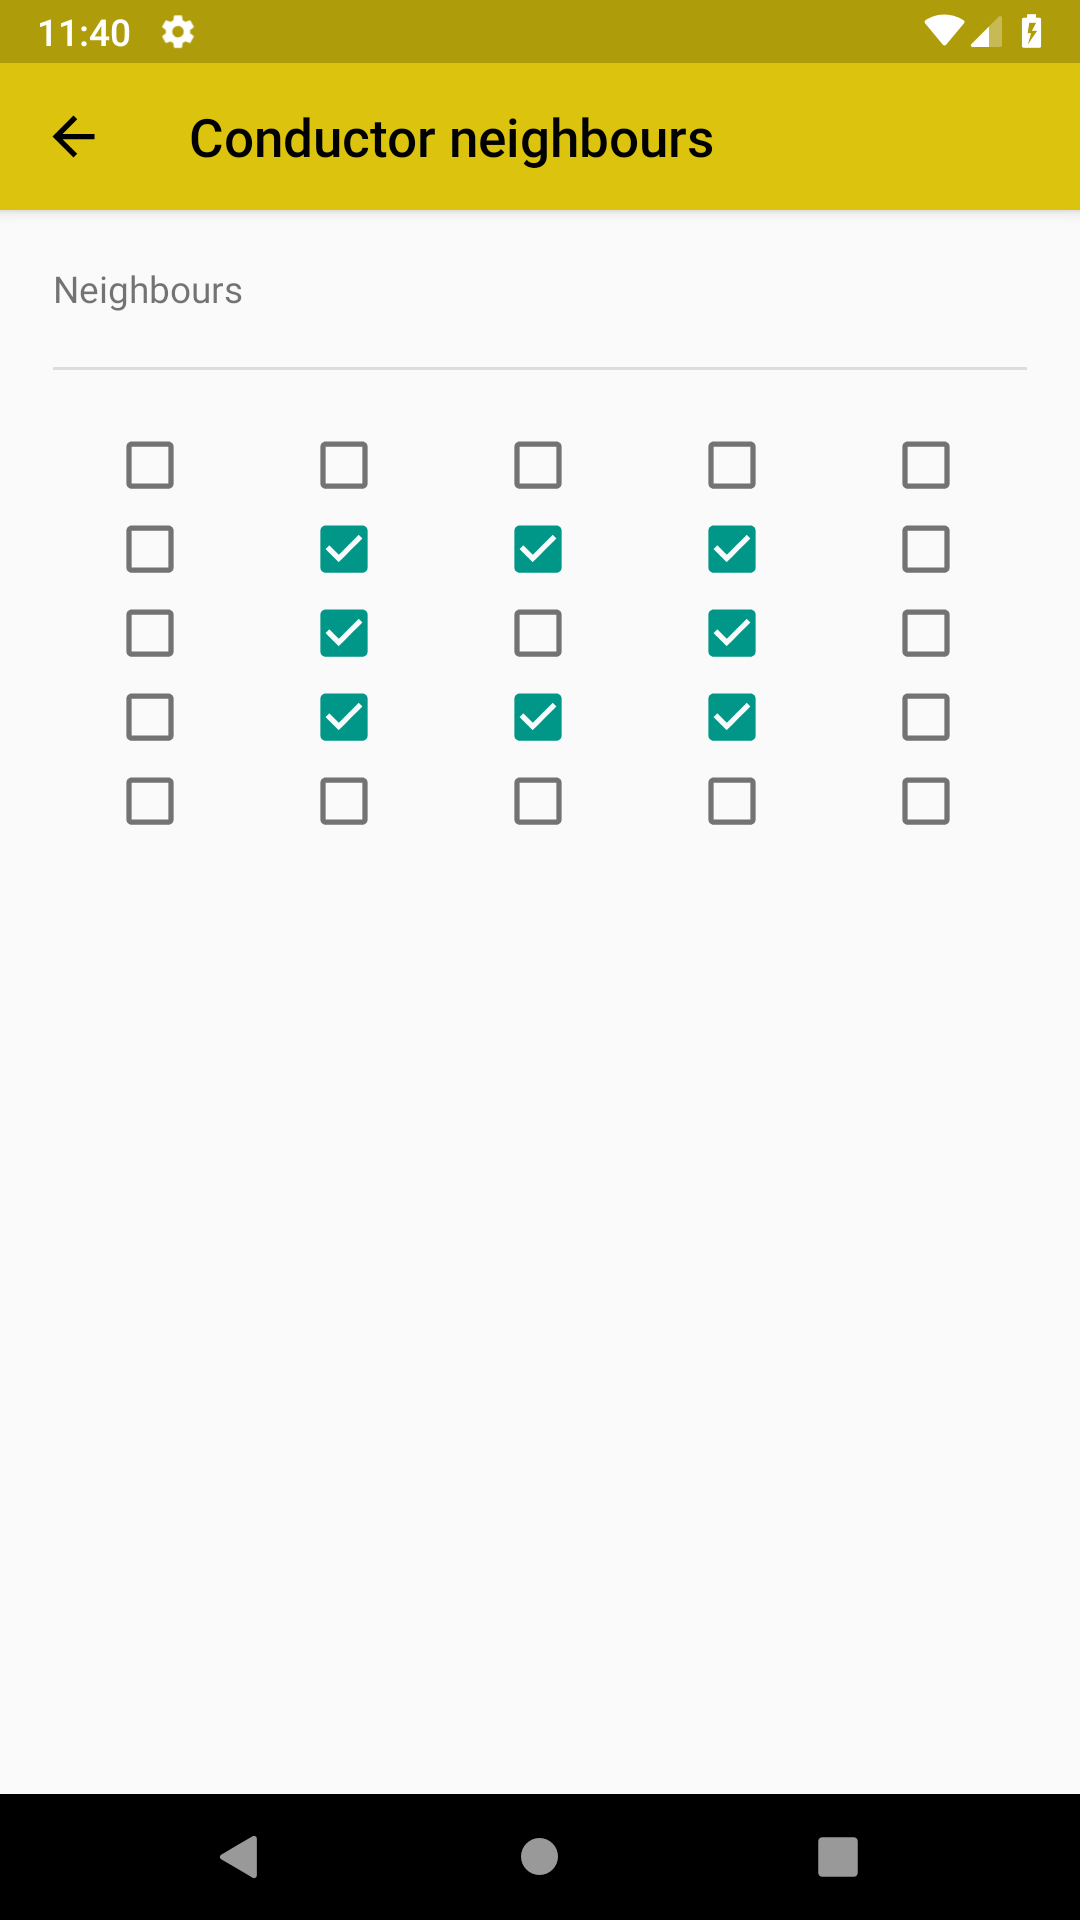
\includegraphics[width=\linewidth]{screens/cell_neighbours.png}
  \end{minipage}\hfill
\end{minipage}
\vspace{20pt}
\begin{minipage}{.45\textwidth}
  \begin{minipage}{.45\linewidth}
    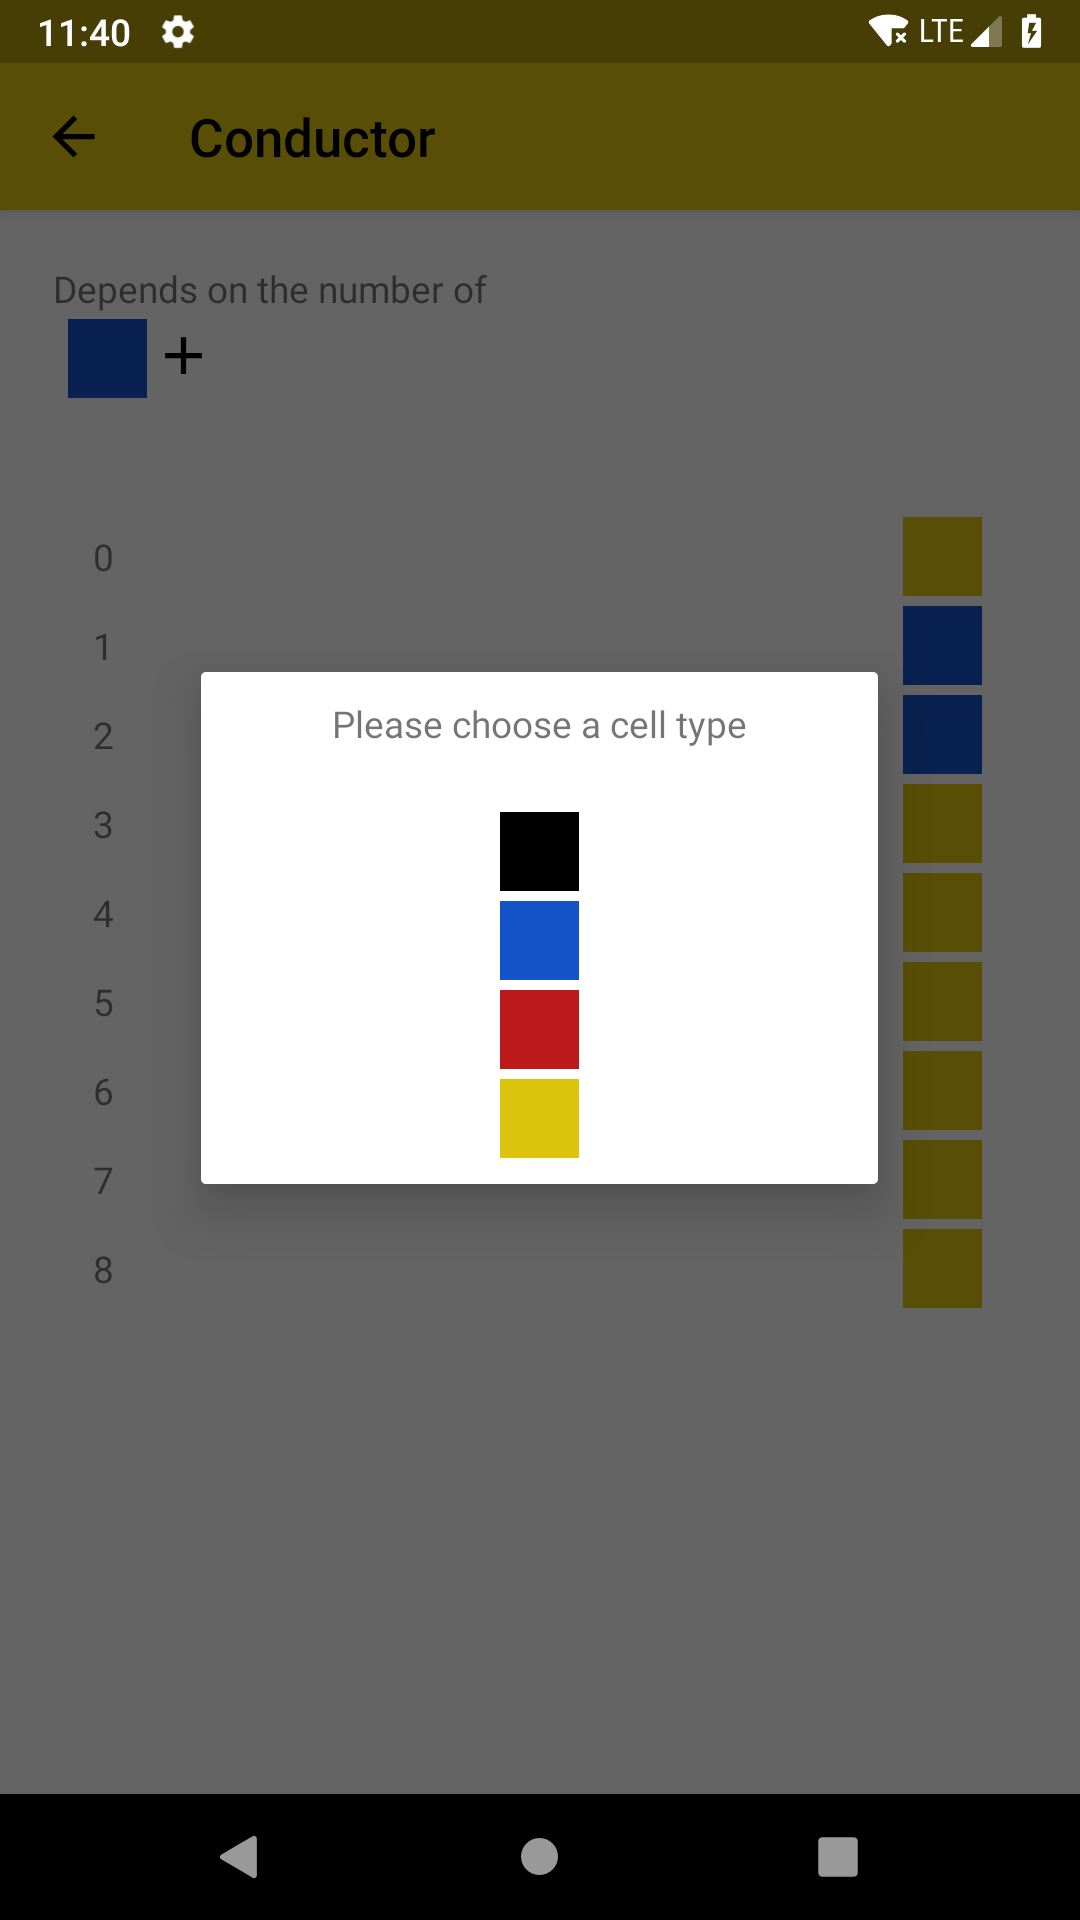
\includegraphics[width=\linewidth]{screens/cell_configuration.png}
  \end{minipage}\hfill
  \begin{minipage}{.45\linewidth}
    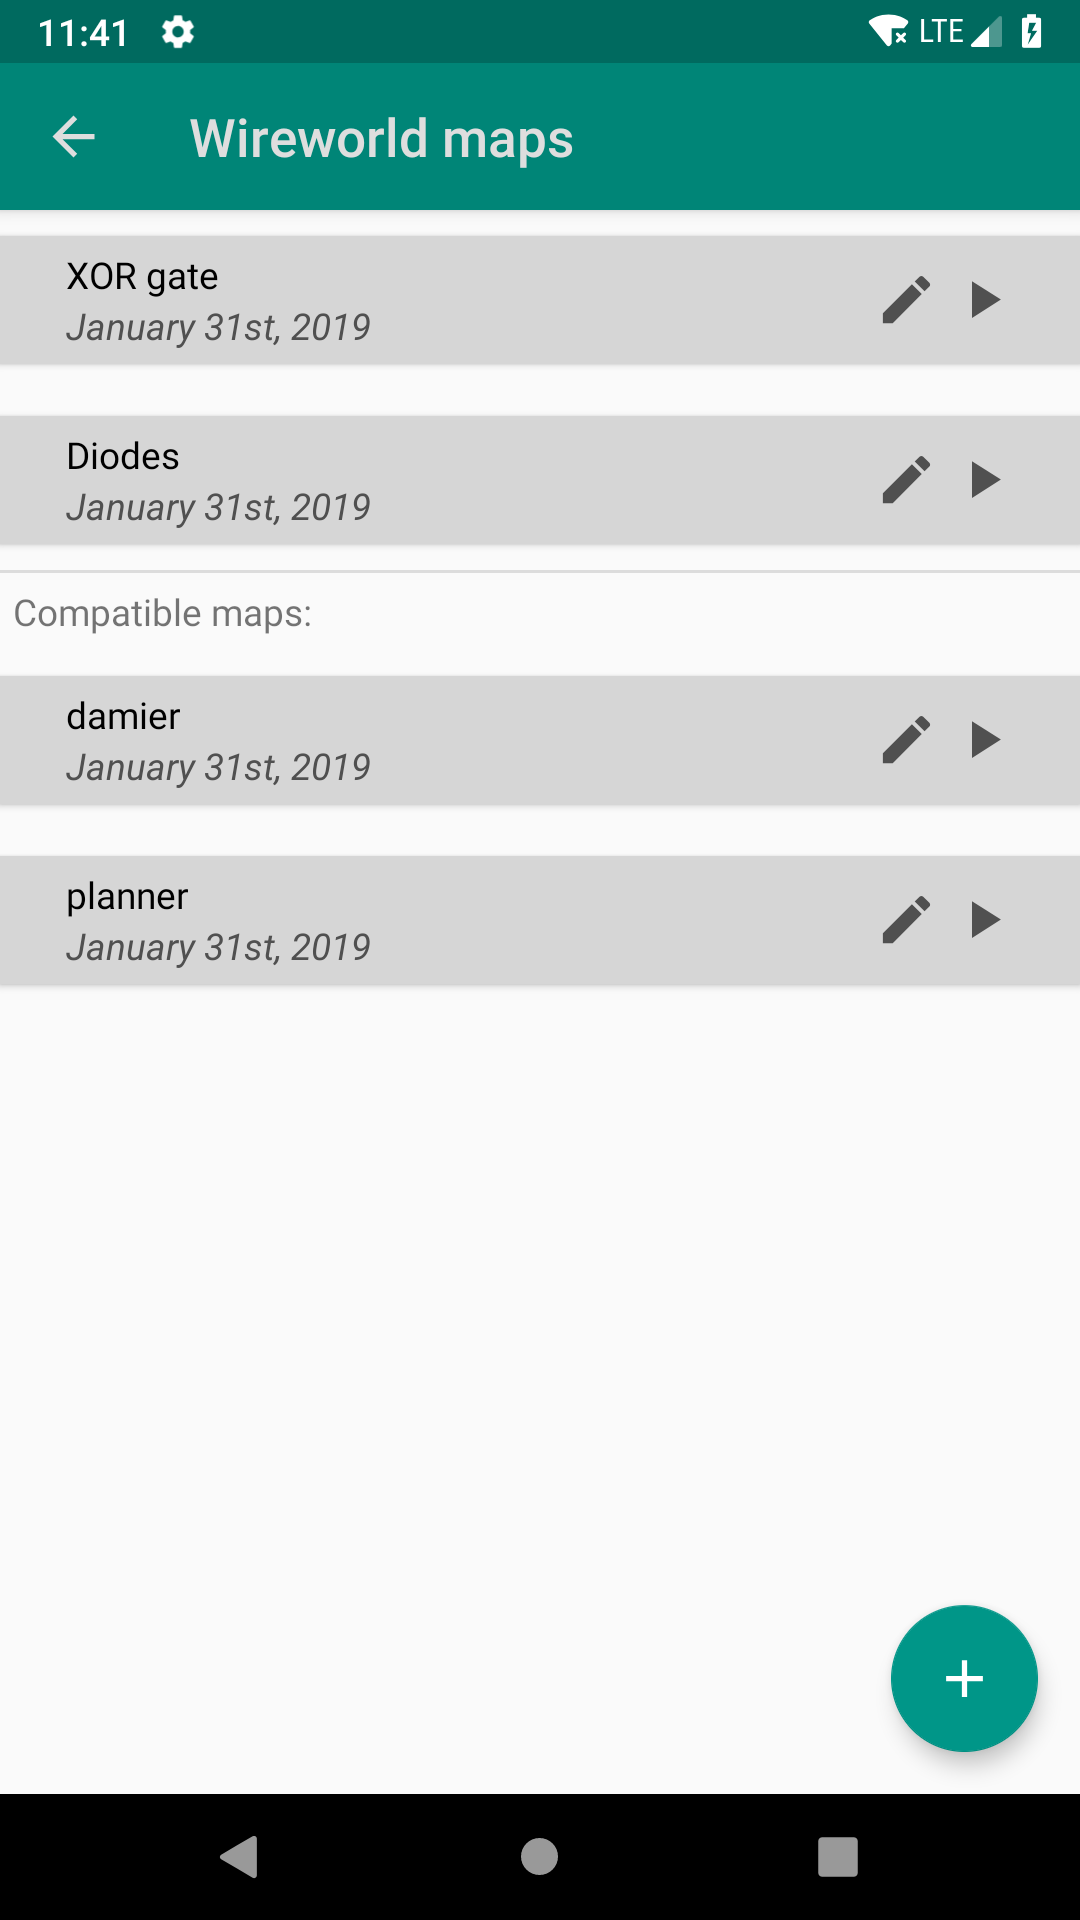
\includegraphics[width=\linewidth]{screens/maps.png}
  \end{minipage}\hfill
\end{minipage} \hfill
\begin{minipage}{.45\textwidth}
  \begin{minipage}{.45\linewidth}
    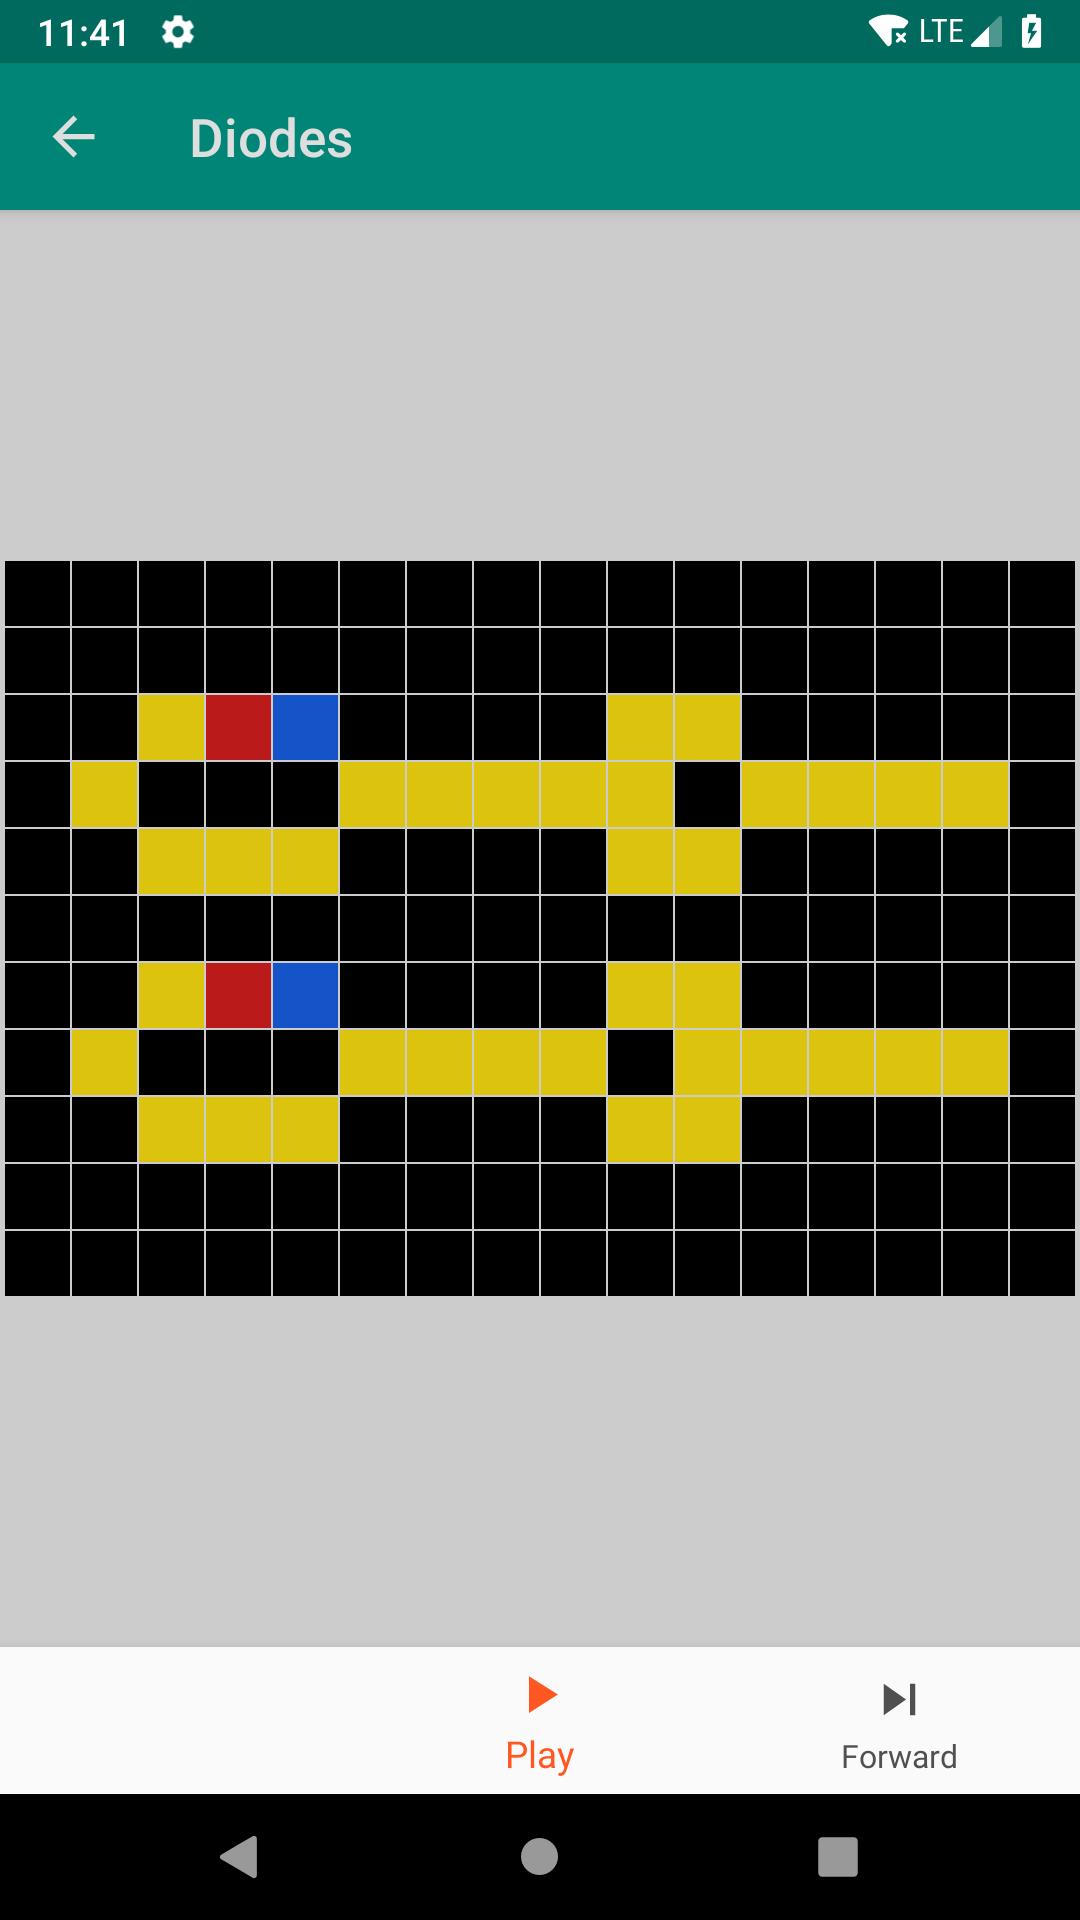
\includegraphics[width=\linewidth]{screens/wireworld.png}
  \end{minipage}\hfill
  \begin{minipage}{.45\linewidth}
    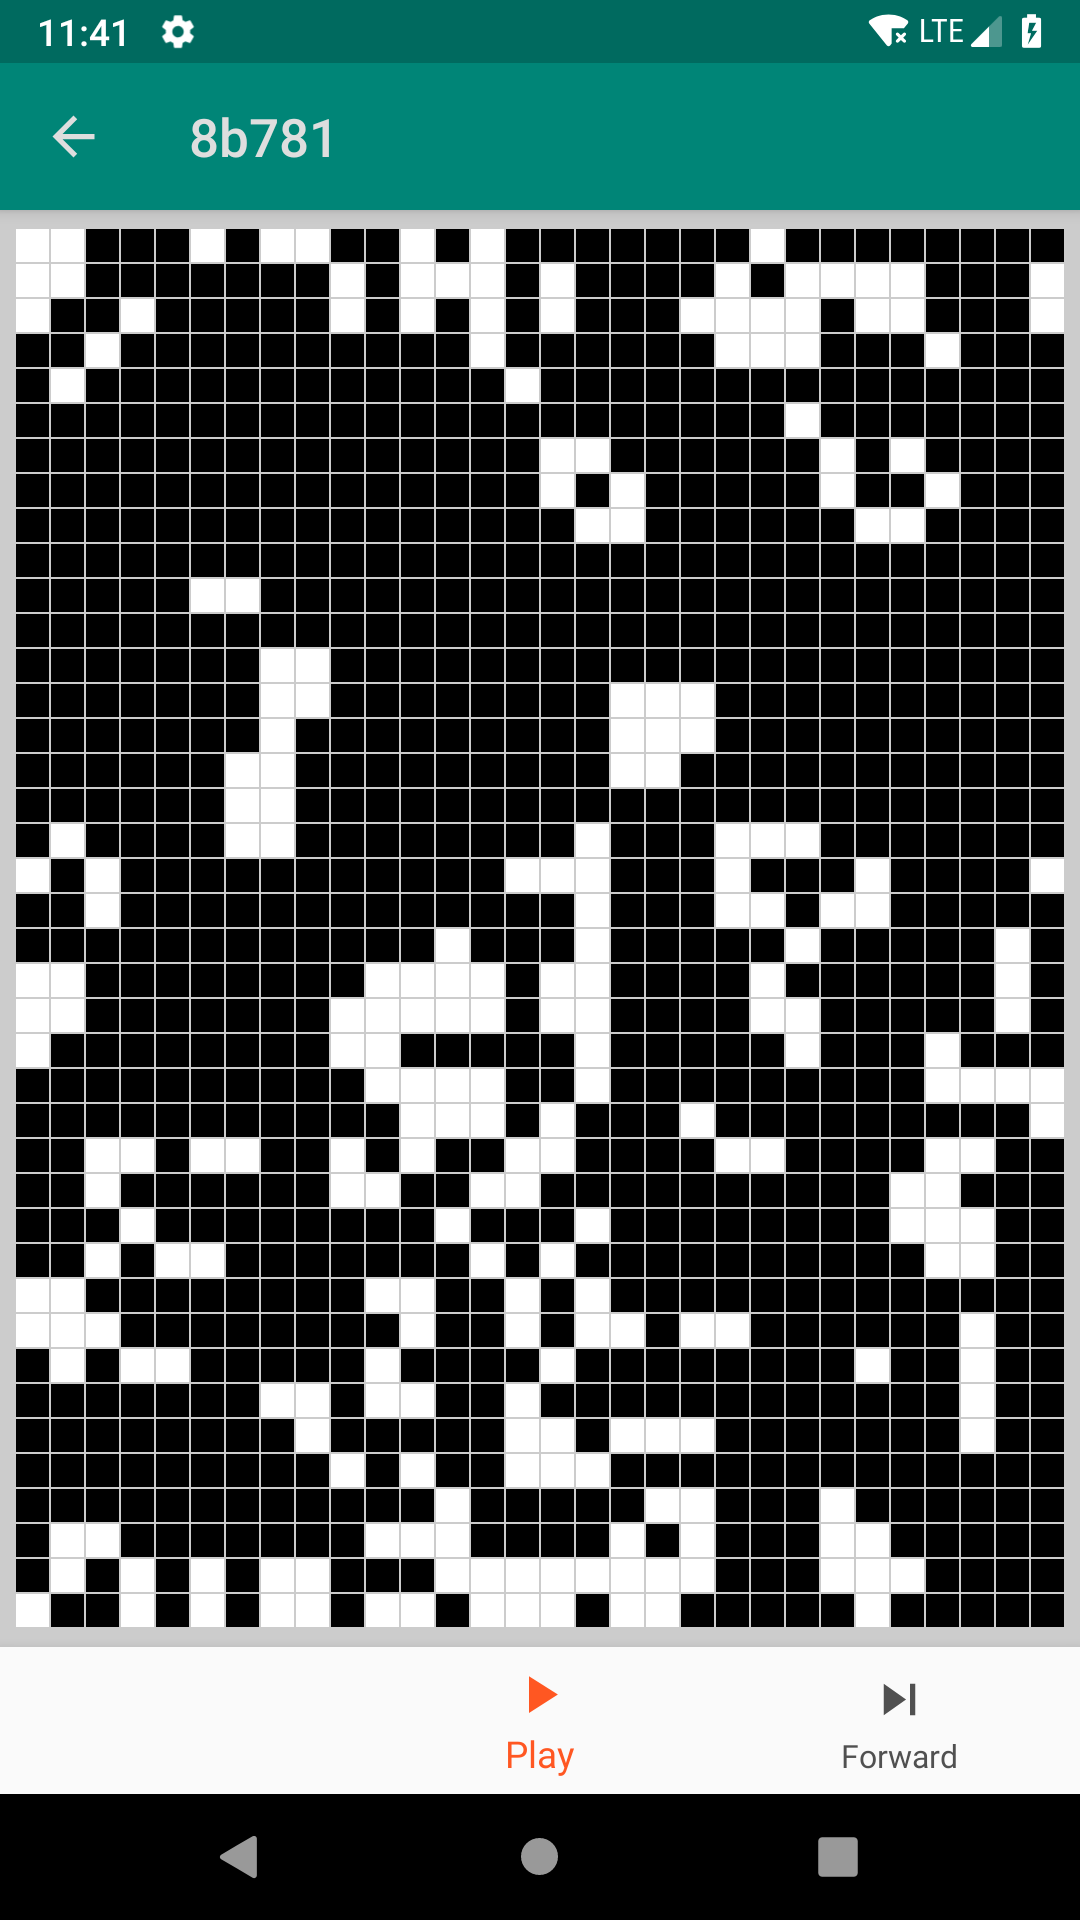
\includegraphics[width=\linewidth]{screens/gameoflife.png}
  \end{minipage}\hfill
\end{minipage} \hfill

\end{document}